A Bayesian network with structure and parameters learned from the training dataset reached an average of \ac{auroc} of 0.89. The results are in the table \ref{tab:result_auc}.

\begin{table}[htbp] 
 \caption{Validation Results (Column AUROC)} 
 \label{tab:result_auc} 

\renewcommand{\arraystretch}{1.2}
\setlength{\tabcolsep}{18pt}

\begin{tabularx}{\textwidth} { X X X X  }
\hline
IA & 0.674 & AA & 0.787 \\
PI & 0.873 & TP & 0.868 \\
IMC & 0.872 & A30 & 0.863 \\
NRCPN & 0.703 & GR & 0.936 \\
IGA & 0.955 & ANP & 1.000 \\
SGP & 0.962 & VCS & 0.730 \\
EPC30 & 0.946 & TG & 0.836 \\
APARA & 0.989 & TPEE & 0.842 \\
AGESTA & 0.931 & V & 0.987 \\
EA & 0.993 & VNH & 0.849 \\
VA & 0.962 & TPNP & 0.928 \\
FA & 0.962 & VP & 0.793 \\
CA & 0.998 &  \\
\hline
 \multicolumn{4}{c}{\textbf{Average}  \textbf{0.890}} \\

\hline
\end{tabularx}
\end{table}


The network is as represented in figure \ref{fig:network}.
%TC:ignore
\begin{figure}[htbp]
\centering
\caption{Network learned}\label{fig:network} 
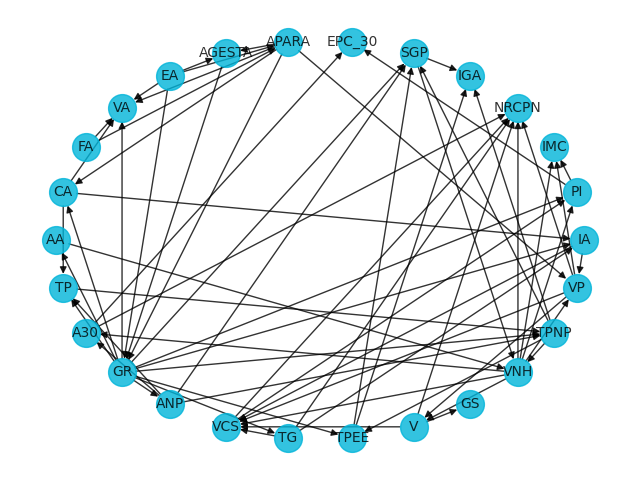
\includegraphics[scale=0.68]{figures/network.png}
\end{figure}
%TC:endignore

As for the rules created, they were conformance based, like the format of dates, and conformance to the value set (i.e. Robson group, bishop scores, or delivery types). We also added plausibility rules, like expected values for BMI, weight and gestational age. We also added plausibility for the relationship between columns, namely weight across different weeks of gestation. We added a relationship of greatness between weights more than 5 weeks apart. 





\subsubsection{Deployment \& Validation} 
The purpose of this model is to be served as an API for usage within a healthcare institution and act as a supplementary decision support tool for obstetrics teams. Although a concrete, vendor-specific information model and health information system were initially used, our goal is to develop a more universal clinical decision support system. This system should be usable across all systems involved in birth and obstetrics departments. Therefore, we constructed it using the \ac{hl7} \ac{fhir}  R5 version standard. This approach simplifies the process of \ac{api} interaction.
Rather than utilizing a proprietary model for the data, we based our decision on the use of \ac{fhir} resources: Bundle and Observation. These resources handle the request and response through a customized operation named "\$quality\_check". Our intention is to publish the profiles of these objects to streamline API access via standardized mechanisms and data models. The current version of the profiles can be accessed at this URL: \url{https://joofio.github.io/obs-cdss-fhir/}. 


For validation, we deployed the tool in docker format in a hospital to gather new data. We gathered 3231 new cases and returned a score for quality as exemplified in figure \ref{fig:scores}. Being that the score is from 0 to 1, the average score was 0.12 and \acp{iqr} was 0.15. We also used the clinician from one of the hospitals that we get data from and asked this clinician to assess 10 records in terms of quality. We gathered the 10 records at random and asked the clinician to assess them in terms of quality. Our purpose was then to compare the rankings of each evaluator; the model and the clinician, in order to assess how similar they were.



%TC:ignore
\begin{figure}[htbp]
\centering
\caption{Scores}\label{fig:scores} 
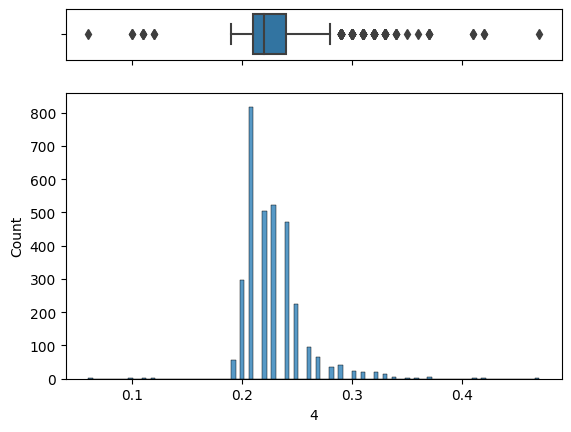
\includegraphics[scale=0.78]{figures/Scoring.png}
\end{figure}
%TC:endignore
